Die früheren Kapitel beschreiben mittels Objektendiagramm die Struktur der Anwendungen nach dem Starten.
Die Schichten sind mittels \textbf{Dependency Injection} (siehe Kapitel \ref{DependencyInjection})  miteinander verknüpft.
Beispiel für \textbf{Port}-\textbf{Adapter}-\textbf{Controller} Verbindung:

\begin{figure}[H]
    \centering
    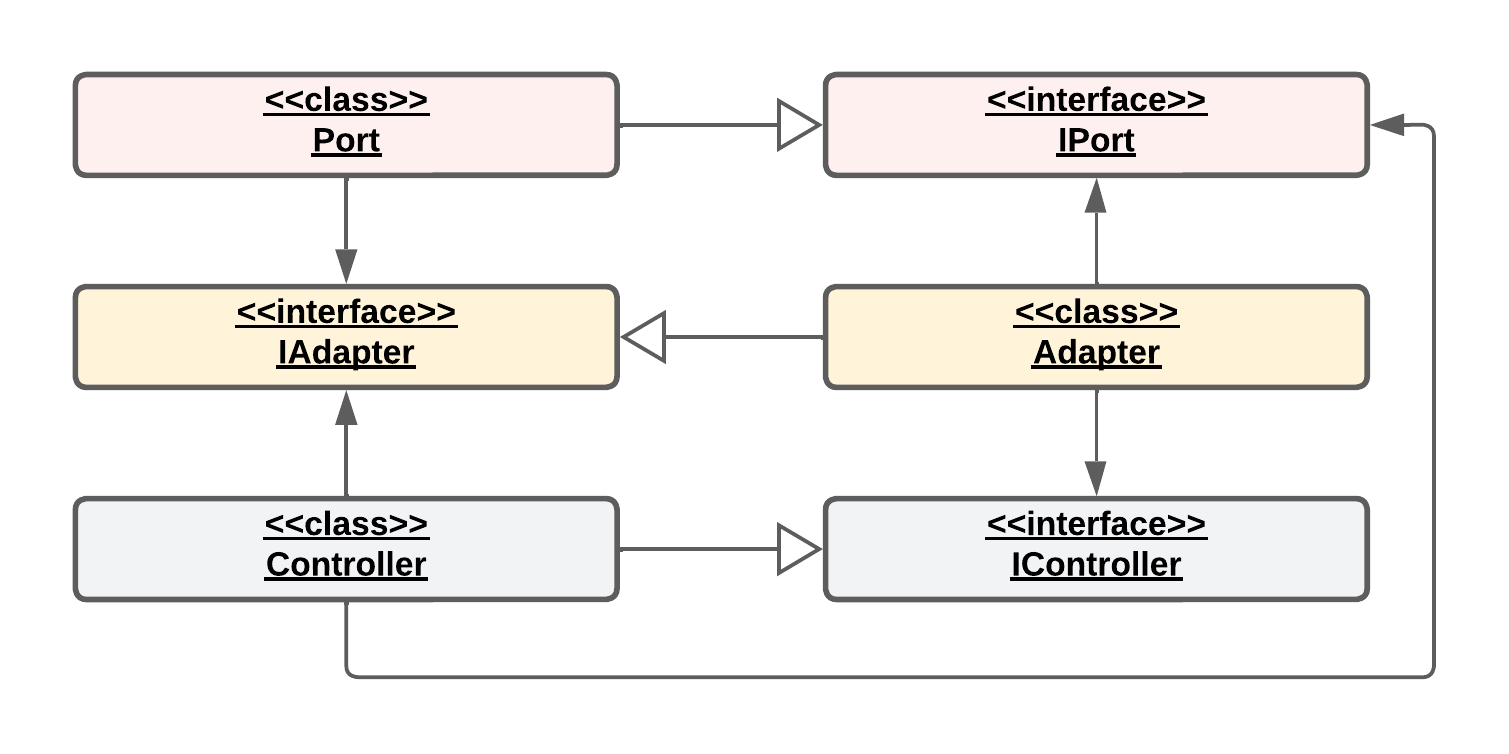
\includegraphics[width=12cm]{./images/Klassendiagramm Port-Adapter.png}
    \caption[Klassendiagramm Port-Adapter-Controller]{Klassendiagramm Port-Adapter-Controller}
    \label{fig:FullCDPAC}
\end{figure}

Beispiele für \textbf{Controller}-\textbf{Dispatcher}-\textbf{UseCase}-\textbf{Interactor} Verbindung:
\begin{figure}[H]
    \centering
    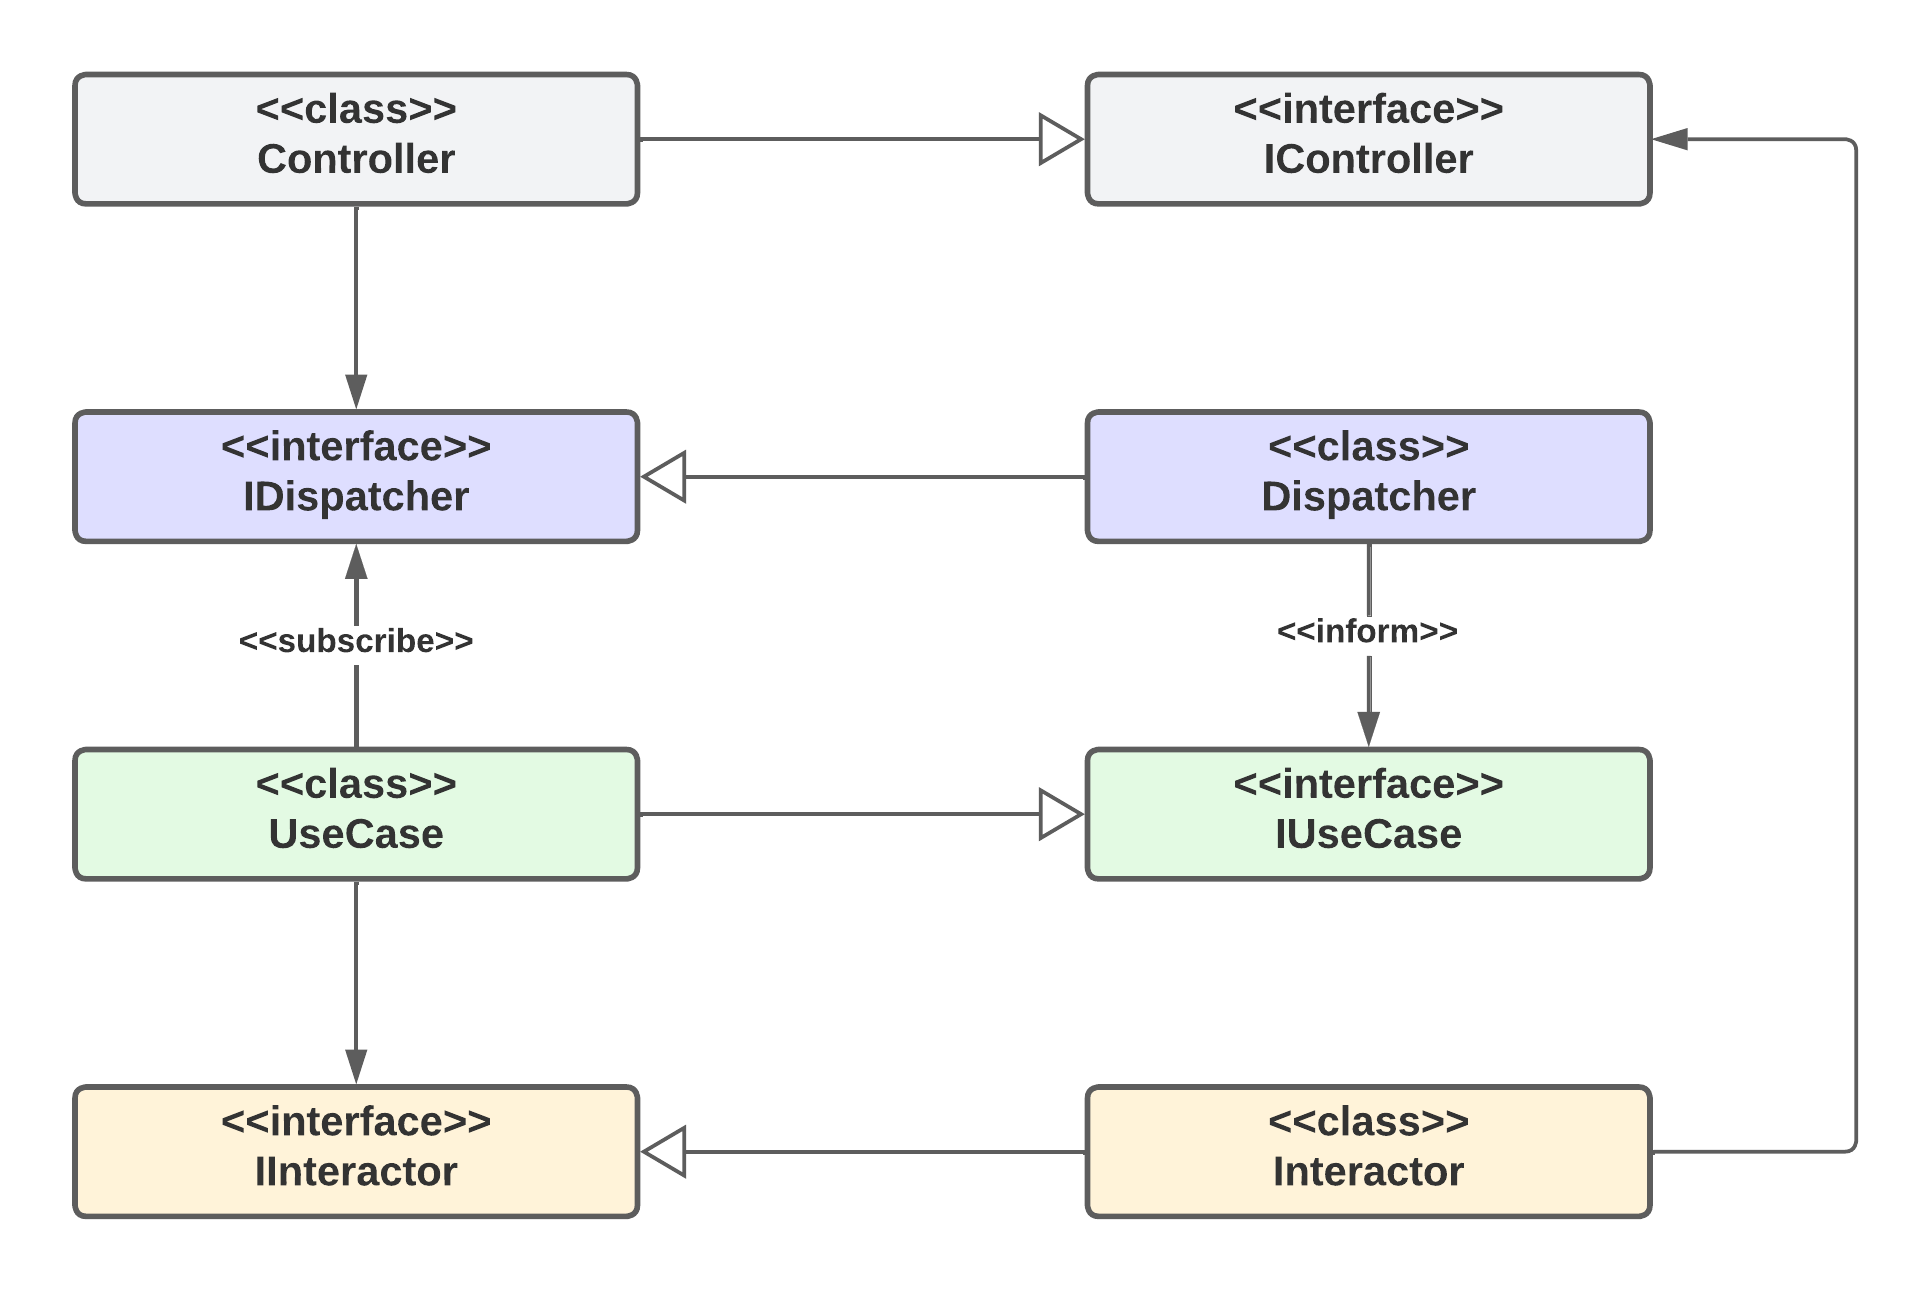
\includegraphics[width=12cm]{./images/CDUI-Klassendiagramm.png}
    \caption[Klassendiagramm Controller-Dispatcher-UseCase-Interactor]{Klassendiagramm Controller-Dispatcher-UseCase-Interactor}
    \label{fig:FullCDCDUI}
\end{figure}

Im Klassendiagramm \ref{fig:FullCDPAC} und \ref{fig:FullCDCDUI} sind alle Klassen miteinander über ein Interface verbunden.
Dies ermöglicht leichte und schnelle Ersetzbarkeit der Schichten und 
somit lässt sich jeder Zustand der Umgebung um einer Schicht simulieren. 
Das ist Voraussetzung für Testbarkeit jeder einzelnen Schicht unabhängig von den anderen Schichten.